\begin{figure}[t]
  \centering

  % pgfplots style "defaultstyle"
  \pgfkeys{/pgfplots/defaultstyle/.style={
      width=1.15\linewidth,
      height=0.25\textheight,
      every axis plot/.append style={line width = 1.2pt},
      every axis plot post/.append style={
        mark size=1, mark options={opacity=0.3}
      },
      tick pos = left,
      xmajorticks = true,
      ymajorticks = true,
      ylabel near ticks,
      xlabel near ticks,
      xtick align = inside,
      ytick align = inside,
      legend cell align = left,
      legend columns = 2,
      legend style = {
        fill opacity = 0.9,
        text opacity = 1,
        font = \tiny,
        at={(0.5,-0.23)},
        anchor=north
      },
      %xticklabel style = {font = \small, inner xsep = 0ex},
      xlabel style = {font = \small},
      axis line style = {black},
      yticklabel style = {font = \small, inner ysep = 0ex},
      ylabel style = {font = \small, inner ysep = 0ex},
      title style = {font = \small, inner ysep = 0ex, yshift = -0.75ex},
      grid = major,
      grid style = {dashed}
    }
  }

\begin{minipage}{0.35\linewidth}
   \pgfkeys{/pgfplots/zmystyle/.style={
    defaultstyle,
    title={$\gL(\vtheta) - \gL(\vtheta_{\text{min}})$},
    ylabel=\empty
    }
  }
   % This file was created by tikzplotlib v0.9.7.
\begin{tikzpicture}

\definecolor{color0}{rgb}{0.12156862745098,0.466666666666667,0.705882352941177}
\definecolor{color1}{rgb}{1,0.498039215686275,0.0549019607843137}

\begin{axis}[
axis line style={white},
legend style={fill opacity=0.8, draw opacity=1, text opacity=1, draw=white!80!black},
log basis x={10},
tick align=outside,
xlabel={Iteration},
xmajorticks=false,
xmin=0.563970595937194, xmax=167345.603972783,
xmode=log,
xtick style={color=white!15!black},
ylabel={Mini-Batch Loss},
ymajorticks=false,
ymin=0.614918631315231, ymax=1.72726913094521,
zmystyle
]
\addplot [, color0]
table {%
0 1.65519058704376
1 1.01682019233704
2 0.780193150043488
3 0.775982201099396
4 0.737731337547302
5 0.771629452705383
6 0.738641858100891
7 0.745266854763031
8 0.772922933101654
9 0.748066663742065
10 0.77786260843277
11 0.769368886947632
12 0.775993466377258
13 0.769854426383972
14 0.780099034309387
15 0.732372939586639
16 0.76972508430481
17 0.77314555644989
18 0.787652790546417
19 0.731954038143158
20 0.753742933273315
21 0.760406374931335
22 0.772047460079193
24 0.752689599990845
25 0.768256425857544
27 0.772502541542053
28 0.745130240917206
30 0.73753297328949
32 0.775065541267395
34 0.7575803399086
36 0.748904526233673
38 0.78914475440979
40 0.774977564811707
42 0.770744025707245
45 0.771463930606842
48 0.724553644657135
51 0.750621318817139
54 0.786653280258179
57 0.740645587444305
60 0.780794203281403
64 0.765990436077118
68 0.772936582565308
72 0.764917433261871
76 0.75068473815918
81 0.763052582740784
86 0.766409575939178
91 0.779118478298187
96 0.779287576675415
102 0.694868266582489
108 0.753131628036499
114 0.745236694812775
121 0.769624173641205
128 0.733922481536865
136 0.763625741004944
144 0.771767735481262
153 0.778103351593018
162 0.76782751083374
172 0.770959913730621
182 0.778098523616791
193 0.747863173484802
204 0.767393231391907
217 0.747031450271606
230 0.761284053325653
243 0.788995981216431
258 0.78480863571167
273 0.725325763225555
289 0.788911044597626
307 0.757820010185242
325 0.701482534408569
344 0.786840677261353
365 0.75093948841095
387 0.793320834636688
410 0.733399331569672
434 0.790173828601837
460 0.789791882038116
488 0.772913932800293
517 0.747723639011383
547 0.767966389656067
580 0.769767463207245
615 0.777678191661835
651 0.732484042644501
690 0.765304982662201
731 0.779313802719116
775 0.752284646034241
821 0.751649916172028
870 0.763818562030792
922 0.763033270835876
977 0.76042252779007
1035 0.794110774993896
1096 0.770817458629608
1162 0.719465613365173
1231 0.773622274398804
1304 0.777041494846344
1382 0.752636194229126
1464 0.746034681797028
1552 0.756577551364899
1644 0.710349500179291
1742 0.788471639156342
1846 0.749858379364014
1956 0.751055300235748
2072 0.77653980255127
2196 0.743179202079773
2327 0.777839779853821
2465 0.765402734279633
2612 0.784416019916534
2768 0.675363481044769
2933 0.767980337142944
3107 0.77206939458847
3292 0.761081337928772
3489 0.780567407608032
3696 0.759546518325806
3917 0.772010743618011
4150 0.731160163879395
4397 0.778384268283844
4659 0.792823255062103
4937 0.780224800109863
5231 0.716187834739685
5542 0.732295513153076
5872 0.757798075675964
6222 0.783280313014984
6593 0.774591028690338
6985 0.76332038640976
7401 0.73084568977356
7842 0.744604051113129
8309 0.77698802947998
8804 0.770139813423157
9329 0.7605100274086
9884 0.745865881443024
10473 0.772988736629486
11097 0.784264206886292
11758 0.73901504278183
12458 0.665480017662048
13200 0.74626225233078
13987 0.765305399894714
14820 0.788454294204712
15702 0.783531785011292
16638 0.790920555591583
17629 0.723659753799438
18679 0.79127299785614
19791 0.776141047477722
20970 0.772833287715912
22219 0.73369562625885
23542 0.771220922470093
24945 0.785363912582397
26430 0.72164660692215
28005 0.788875877857208
29673 0.772274553775787
31440 0.764169812202454
33312 0.723604738712311
35297 0.758412897586823
37399 0.769568562507629
39626 0.782877564430237
41987 0.774317562580109
44487 0.74730920791626
47137 0.759216368198395
49945 0.75877833366394
52919 0.77678370475769
56071 0.770803034305573
59411 0.757794678211212
62949 0.775205314159393
66699 0.787786245346069
70671 0.761527419090271
74881 0.740764439105988
79340 0.766364872455597
84066 0.771571159362793
89073 0.774646580219269
94378 0.766631364822388
};
\addlegendentry{SGD}
\addplot [, color1]
table {%
0 1.67670774459839
1 1.00288474559784
2 0.814482688903809
3 0.769742786884308
4 0.761073589324951
5 0.759601593017578
6 0.759367525577545
7 0.759331345558167
8 0.759325861930847
9 0.759325087070465
10 0.759324848651886
11 0.759324848651886
12 0.759324908256531
13 0.759324848651886
14 0.759324848651886
15 0.759324848651886
16 0.759324848651886
17 0.759324848651886
18 0.759324908256531
19 0.759324848651886
20 0.759324848651886
21 0.759324848651886
22 0.759324848651886
24 0.759324789047241
25 0.759324848651886
27 0.759324848651886
28 0.759324848651886
30 0.759324848651886
32 0.759324848651886
34 0.759324848651886
36 0.759324908256531
38 0.759324848651886
40 0.759324848651886
42 0.759324848651886
45 0.759324908256531
48 0.759324848651886
51 0.759324848651886
54 0.759324848651886
57 0.759324848651886
60 0.759324848651886
64 0.759324848651886
68 0.759324848651886
72 0.759324848651886
76 0.759324848651886
81 0.759324908256531
86 0.759324789047241
91 0.759324848651886
96 0.759324908256531
102 0.759324848651886
108 0.759324848651886
114 0.759324908256531
121 0.759324848651886
128 0.759324848651886
136 0.759324789047241
144 0.759324908256531
153 0.759324848651886
162 0.759324848651886
172 0.759324908256531
182 0.759324908256531
193 0.759324848651886
204 0.759324908256531
217 0.759324908256531
230 0.759324908256531
243 0.759324848651886
258 0.759324848651886
273 0.759324908256531
289 0.759324848651886
307 0.759324848651886
325 0.759324848651886
344 0.759324789047241
365 0.759324848651886
387 0.759324848651886
410 0.759324908256531
434 0.759324848651886
460 0.759324848651886
488 0.759324848651886
517 0.759324848651886
547 0.759324848651886
580 0.759324908256531
615 0.759324908256531
651 0.759324848651886
690 0.759324848651886
731 0.759324848651886
775 0.759324789047241
821 0.759324848651886
870 0.759324848651886
922 0.759324848651886
977 0.759324848651886
1035 0.759324908256531
1096 0.759324908256531
1162 0.759324789047241
1231 0.759324848651886
1304 0.759324848651886
1382 0.759324848651886
1464 0.759324848651886
1552 0.759324848651886
1644 0.759324848651886
1742 0.759324908256531
1846 0.759324848651886
1956 0.759324908256531
2072 0.759324908256531
2196 0.759324908256531
2327 0.759324789047241
2465 0.759324908256531
2612 0.759324848651886
2768 0.759324848651886
2933 0.759324848651886
3107 0.759324848651886
3292 0.759324908256531
3489 0.759324908256531
3696 0.759324908256531
3917 0.759324848651886
4150 0.759324848651886
4397 0.759324848651886
4659 0.759324848651886
4937 0.759324848651886
5231 0.759324848651886
5542 0.759324848651886
5872 0.759324908256531
6222 0.759324908256531
6593 0.759324848651886
6985 0.759324908256531
7401 0.759324908256531
7842 0.759324848651886
8309 0.759324848651886
8804 0.759324908256531
9329 0.759324848651886
9884 0.759324908256531
10473 0.759324848651886
11097 0.759324908256531
11758 0.759324848651886
12458 0.759324848651886
13200 0.759324848651886
13987 0.759324908256531
14820 0.759324908256531
15702 0.759324848651886
16638 0.759324848651886
17629 0.759324848651886
18679 0.759324908256531
19791 0.759324908256531
20970 0.759324848651886
22219 0.759324848651886
23542 0.759324848651886
24945 0.759324848651886
26430 0.759324908256531
28005 0.759324848651886
29673 0.759324848651886
31440 0.759324789047241
33312 0.759324848651886
35297 0.759324848651886
37399 0.759324789047241
39626 0.759324908256531
41987 0.759324848651886
44487 0.759324848651886
47137 0.759324848651886
49945 0.759324848651886
52919 0.759324848651886
56071 0.759324848651886
59411 0.759324908256531
62949 0.759324789047241
66699 0.759324848651886
70671 0.759324848651886
74881 0.759324848651886
79340 0.759324848651886
84066 0.759324848651886
89073 0.759324848651886
94378 0.759324908256531
};
\addlegendentry{GD}
\end{axis}

\end{tikzpicture}

\end{minipage}
%
\begin{minipage}{0.38\linewidth}
  \pgfkeys{/pgfplots/zmystyle/.style={
    defaultstyle,
    title={$\Vert \vtheta - \vtheta_{\text{min}} \Vert$ after $20$ steps},
    ylabel=\empty,
    xlabel=\phantom{step},
    xtick=\empty,
    xtick={0, 1, 2, 3, 4, 5, 6, 7, 8},
    xticklabels={SGD, $\delta_k$ (ours), $\delta=10^{-4}$, $\delta=10^{-3}$,
    $\delta=10^{-2}$, $\delta=10^{-1}$, $\delta=10^{0}$, $\delta=10^{1}$, $\delta=10^{2}$},
    xticklabel style = {font = \tiny, rotate = 75, anchor = east, inner xsep = 1 ex}
    }
  }
   \input{../../fig/exp09_noisy_quadratic/Distance_at_end.tex}
\end{minipage}
%
\begin{minipage}{0.25\linewidth}
  \pgfkeys{/pgfplots/zmystyle/.style={defaultstyle,
    title={Relative damping $\nicefrac{\delta_k}{k^2}$},
    ylabel=\empty
    }
  }
   \input{../../fig/exp09_noisy_quadratic/Dampings.tex}
   \vspace{9.5mm}
\end{minipage}

\vspace{-2.0ex}
\caption{\textbf{Comparison of optimizers on noisy quadratic.} Statistics for
  different optimizers during (\textit{left}) and at the end (\textit{center})
  of training over $100$ runs. For the loss values, we present mean (dashed
  line), median (solid line) and a confidence interval (shaded area) between the
  lower and upper quartile. Boxplot whiskers range from the distribution's
  minimum to the maximum and boxes indicate lower and upper quartile, enclosing
  the median. Horizontal black lines indicate the initial loss/distance.
  \textit{Right}: Relative dampings of our adaptive method. Darker shades
  indicate larger curvatures.}
  \label{fig:noisy_quadratic}
\end{figure}

%%% Local Variables:
%%% mode: latex
%%% TeX-master: "../main"
%%% End:
